\chapter{الذرات والجزيئات}\label{ch:g7:atoms-and-molecules}

خذ قطرة ماء واقسمها نصفين. كل نصف لا يزال ماءً. اقسم نصفًا منهما من
جديد، ثم مرة أخرى، ومرة أخرى. هل تستطيع أن تستمر إلى ما لا نهاية، أم
ستبلغ قطعة صغيرة إلى حد أن قسمتها مرة أخرى تعطي شيئًا لم يعد ماءً
أبدًا؟ نحو سنة 400 قبل الميلاد خمّن المفكر الإغريقي ديموقريطس الجواب:
المادة مكوّنة من قطع دقيقة لا تنقسم، سماها \emph{\omterm{def:g7:atoms-and-molecules:atom}{الذرات}}، من الكلمة
الإغريقية التي تعني «ما لا ينقسم». واحتاج الأمر إلى أكثر من ألفي سنة،
وإلى عمل كيميائيي القرن التاسع عشر، حتى يصير ذلك التخمين علمًا. يصف هذا
الفصل هذه القطع --- \omterm{def:g7:atoms-and-molecules:atom}{الذرات} --- وكيف تتجمع في \omterm{def:g7:atoms-and-molecules:molecule}{جزيئات}.

\begin{recall}
\omterm{def:g6:pure-substances-and-mixtures:pure-substance}{المادة النقية}، مثل الماء أو الأكسجين، مكوّنة من \omterm{def:g6:pure-substances-and-mixtures:species}{نوع كيميائي} واحد؛ أما
\omterm{def:g6:pure-substances-and-mixtures:mixture}{الخليط}، مثل \omterm{def:g4:air-a-mixture-of-gases:air}{الهواء}، فيحوي عدة أنواع
(\cref{ch:g6:pure-substances-and-mixtures}). \omterm{def:g4:air-a-mixture-of-gases:air}{والهواء} نحو أربعة أخماسه
نيتروجين وخمسه أكسجين (\cref{ch:g4:air-a-mixture-of-gases}).
\end{recall}

\section{الذرات}

\begin{definition}[الذرة]\label{def:g7:atoms-and-molecules:atom}
كل المادة مبنية من جسيمات بالغة الصغر تسمى
\emph{الذرات}\index{ذرة}. ولا يوجد في الطبيعة إلا نحو مئة نوع مختلف من
الذرات، وكل مادة --- الماء، \omterm{def:g4:air-a-mixture-of-gases:air}{والهواء}، والحديد، والسكر، وأجسامنا نفسها ---
مكوّنة من ذرات من بضعة أنواع منها.
\end{definition}

\begin{proposition}[الذرات بالغة الصغر]\label{prop:g7:atoms-and-molecules:tiny}
% ledger: const:a0, earth:diameter (8 cm apple: 12756 km / 8 cm = 1.6 x 10^8;
% 0.1-0.15 nm x 1.6 x 10^8 = 1.7-2.4 cm, a small cherry)
أصغر \omterm{def:g7:atoms-and-molecules:atom}{الذرات}، \omterm{def:g7:atoms-and-molecules:atom}{ذرة} الهيدروجين، قطرها نحو جزء من عشرة ملايين من
المليمتر؛ \omterm{def:g7:atoms-and-molecules:atom}{والذرات} الأخرى أكبر منها ببضع مرات على الأكثر. فعشرة ملايين \omterm{def:g7:atoms-and-molecules:atom}{ذرة}
هيدروجين متراصفة تصنع خطًا طوله مليمتر واحد. ولتتخيل ذلك: لو كُبّرت تفاحة
حتى تصير في حجم الأرض، لكانت كل \omterm{def:g7:atoms-and-molecules:atom}{ذرة} من ذراتها في حجم كرزة صغيرة
تقريبًا.
\end{proposition}

\begin{remark}[تُرى دون أن تُرى]\label{rem:g7:atoms-and-molecules:seen}
لا يستطيع أي مجهر ضوئي أن يُظهر \omterm{def:g7:atoms-and-molecules:atom}{ذرة}: \omterm{def:g7:atoms-and-molecules:atom}{فالذرات} أصغر بكثير من موجات الضوء.
ومنذ ثمانينيات القرن العشرين صارت مجاهر خاصة، تتحسس السطح برأس بالغ
الدقة، تصنع صورًا تظهر فيها \omterm{def:g7:atoms-and-molecules:atom}{الذرات} المنفردة نتوءاتٍ.
\end{remark}

\begin{definition}[رمز الذرة]\label{def:g7:atoms-and-molecules:symbol}
لكل نوع من \omterm{def:g7:atoms-and-molecules:atom}{الذرات} اسم و\emph{رمز}\index{رمز الذرة}: حرف لاتيني كبير
واحد، يتبعه أحيانًا حرف صغير واحد. والرمز واحد في كل
اللغات.
\end{definition}

\begin{center}
\small
\begin{tabular}{llll|llll}
\hline
\omterm{def:g7:atoms-and-molecules:atom}{الذرة} & \omterm{def:g7:atoms-and-molecules:symbol}{الرمز} & & لون النموذج & \omterm{def:g7:atoms-and-molecules:atom}{الذرة} & \omterm{def:g7:atoms-and-molecules:symbol}{الرمز} & & لون النموذج \\
\hline
الهيدروجين & \ce{H} & \tikz\node[aH]{}; & أبيض & الصوديوم & \ce{Na} & \tikz\node[aNa]{}; & بنفسجي \\
الكربون & \ce{C} & \tikz\node[aC]{}; & أسود & الكبريت & \ce{S} & \tikz\node[aS]{}; & أصفر \\
النيتروجين & \ce{N} & \tikz\node[aN]{}; & أزرق & الكلور & \ce{Cl} & \tikz\node[aCl]{}; & أخضر \\
الأكسجين & \ce{O} & \tikz\node[aO]{}; & أحمر & الحديد، النحاس & \ce{Fe}، \ce{Cu} & & --- \\
\hline
\end{tabular}
\end{center}

\begin{remark}[من أين تأتي الرموز]\label{rem:g7:atoms-and-molecules:latin}
معظم الرموز هي الحروف الأولى من الاسم الدولي \omterm{def:g7:atoms-and-molecules:atom}{للذرة}: \ce{H} للهيدروجين،
و\ce{C} للكربون، و\ce{O} للأكسجين. وبعضها مأخوذ من اسم لاتيني أقدم:
\ce{Na} للصوديوم (\emph{natrium})، و\ce{Fe} للحديد
(\emph{ferrum})، و\ce{Cu} للنحاس (\emph{cuprum}). والحرف الثاني صغير
دائمًا: \ce{Co} \omterm{def:g7:atoms-and-molecules:atom}{ذرة} الكوبالت، أما CO، بحرف O كبير، فشيء آخر
تمامًا.
\end{remark}

\begin{history}[ذرات دالتون، 1808]
نشر الكيميائي جون دالتون سنة 1808 جدولًا \omterm{def:g7:atoms-and-molecules:atom}{للذرات} المعروفة في زمنه، رسم
كل واحدة منها دائرة صغيرة لها علامتها الخاصة. وكان أول من قال إن كل \omterm{def:g7:atoms-and-molecules:atom}{ذرات}
النوع الواحد لها الوزن نفسه، وإن الكيميائيين يستطيعون مقارنة هذه الأوزان.
لكنه خمّن أيضًا أن الماء \omterm{def:g7:atoms-and-molecules:atom}{ذرة} هيدروجين واحدة مرتبطة \omterm{def:g7:atoms-and-molecules:atom}{بذرة} أكسجين واحدة؛
واحتاج الكيميائيون إلى خمسين سنة أخرى ليتفقوا على أن \omterm{def:g7:atoms-and-molecules:molecule}{جزيء} الماء يحوي
\emph{ذرتي} هيدروجين.
\end{history}

\begin{omfigure}
\begin{minipage}[b]{0.3\linewidth}\centering
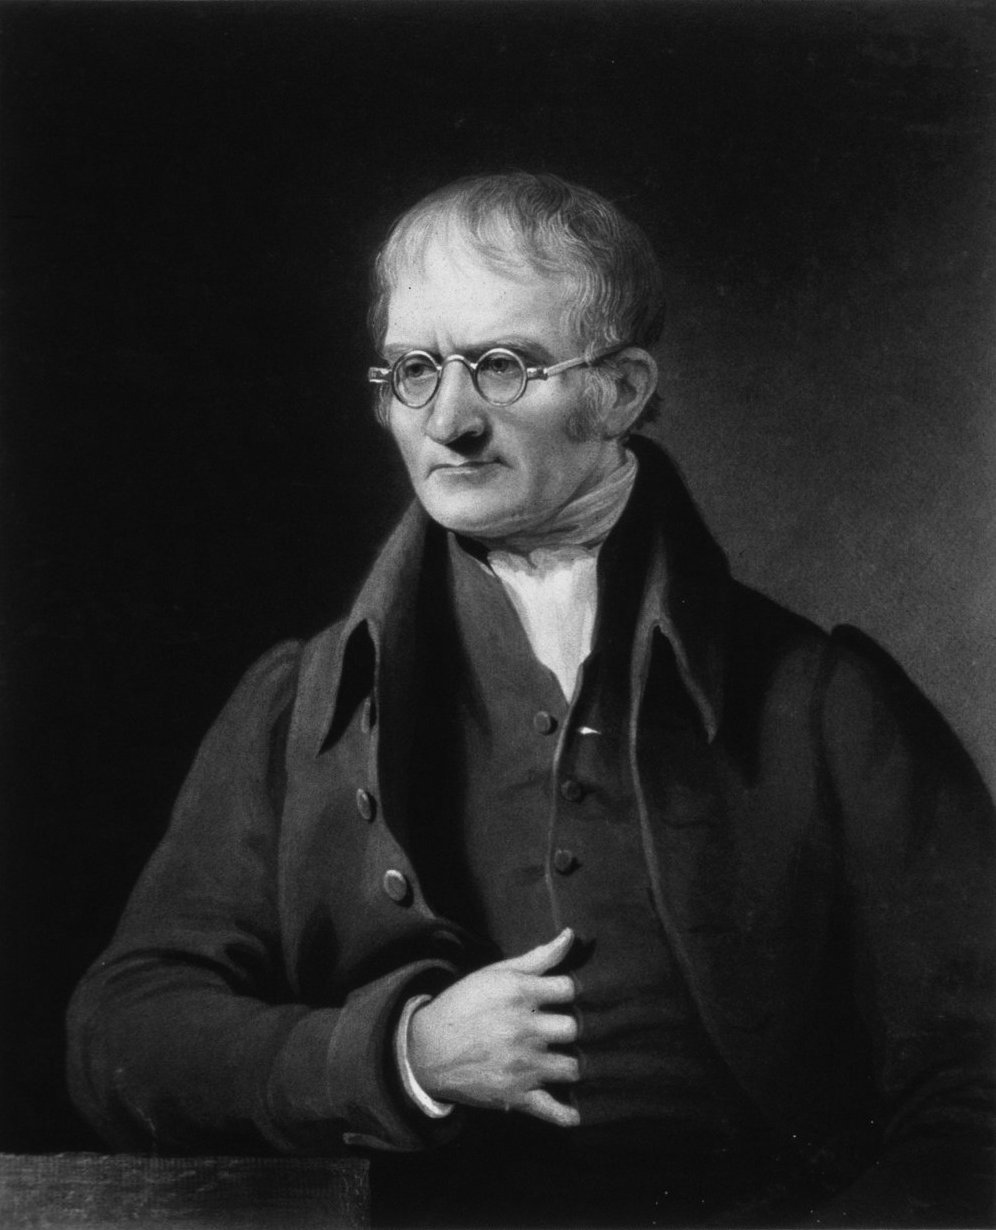
\includegraphics[width=\linewidth]{images/book1/dalton.jpg}

{\small جون دالتون (1766--1844).}
\end{minipage}\hfill
\begin{minipage}[b]{0.66\linewidth}\centering
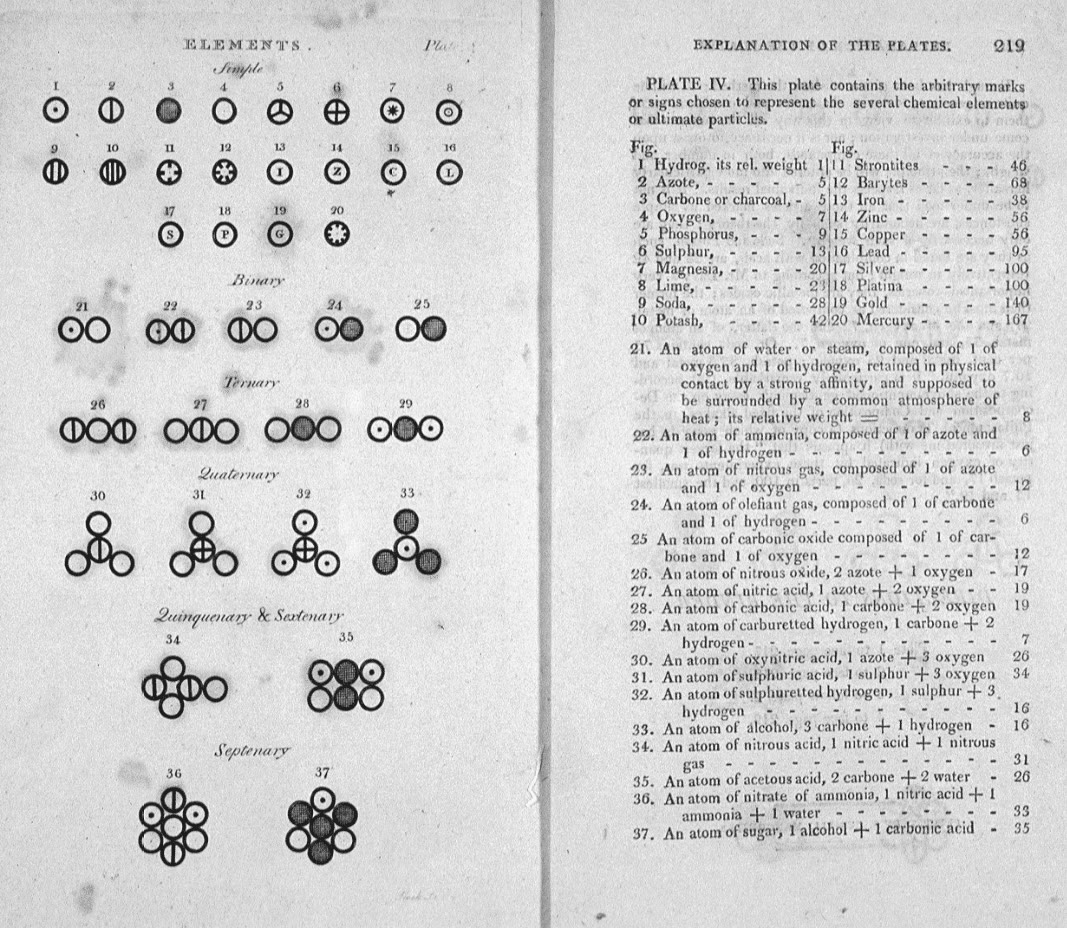
\includegraphics[width=\linewidth]{images/book1/dalton-symbols.jpg}

{\small جدول دالتون لسنة 1808: الماء عنده، العلامة 21، دائرة هيدروجين
بجانب دائرة أكسجين.}
\end{minipage}
\end{omfigure}

\section{الجزيئات}

\begin{definition}[الجزيء]\label{def:g7:atoms-and-molecules:molecule}
\emph{الجزيء}\index{جزيء} مجموعة من \omterm{def:g7:atoms-and-molecules:atom}{الذرات} مرتبط بعضها ببعض ارتباطًا
وثيقًا. والجزيء أصغر قطعة من مادة تبقى هي تلك المادة: فجزيء الماء أصغر
مقدار ممكن من الماء.
\end{definition}

\begin{example}[سبعة جزيئات]\label{ex:g7:atoms-and-molecules:seven}
\begin{itemize}
  \item \omterm{def:g7:atoms-and-molecules:molecule}{جزيء} \emph{الهيدروجين}: ذرتا هيدروجين؛
  \item \omterm{def:g7:atoms-and-molecules:molecule}{جزيء} \emph{الأكسجين}، الذي نتنفسه: ذرتا أكسجين؛
  \item \omterm{def:g7:atoms-and-molecules:molecule}{جزيء} \emph{النيتروجين}، أربعة أخماس \omterm{def:g4:air-a-mixture-of-gases:air}{الهواء}: ذرتا
        نيتروجين؛
  \item \omterm{def:g7:atoms-and-molecules:molecule}{جزيء} \emph{الماء}: ذرتا هيدروجين \omterm{def:g7:atoms-and-molecules:atom}{وذرة} أكسجين
        واحدة؛
  \item \omterm{def:g7:atoms-and-molecules:molecule}{جزيء} \emph{ثنائي أكسيد الكربون}، الذي نزفره: \omterm{def:g7:atoms-and-molecules:atom}{ذرة}
        كربون واحدة وذرتا أكسجين؛
  \item \omterm{def:g7:atoms-and-molecules:molecule}{جزيء} \emph{الميثان}، المكوّن الرئيسي للغاز الطبيعي الذي
        يُحرق في مواقد الغاز: \omterm{def:g7:atoms-and-molecules:atom}{ذرة} كربون واحدة وأربع \omterm{def:g7:atoms-and-molecules:atom}{ذرات} هيدروجين؛
  \item \omterm{def:g7:atoms-and-molecules:molecule}{جزيء} \emph{أكسيد النيتروز}، وهو غاز مخدّر: ذرتا
        نيتروجين \omterm{def:g7:atoms-and-molecules:atom}{وذرة} أكسجين واحدة.
\end{itemize}
\end{example}

\begin{omfigure}
\begin{tikzpicture}[font=\small]
  % hydrogen
  \begin{scope}[xshift=0cm]
    \node[aH] (a) at (-0.25,0) {}; \node[aH] (b) at (0.25,0) {};
    \begin{scope}[on background layer]\draw[bond] (a.center) -- (b.center);\end{scope}
    \node at (0,-1.05) {الهيدروجين};
  \end{scope}
  % oxygen
  \begin{scope}[xshift=2.6cm]
    \node[aO] (a) at (-0.33,0) {}; \node[aO] (b) at (0.33,0) {};
    \begin{scope}[on background layer]
      \draw[bond, line width=1.1pt] ([yshift=1.6pt]a.center) -- ([yshift=1.6pt]b.center);
      \draw[bond, line width=1.1pt] ([yshift=-1.6pt]a.center) -- ([yshift=-1.6pt]b.center);
    \end{scope}
    \node at (0,-1.05) {الأكسجين};
  \end{scope}
  % nitrogen
  \begin{scope}[xshift=5.2cm]
    \node[aN] (a) at (-0.33,0) {}; \node[aN] (b) at (0.33,0) {};
    \begin{scope}[on background layer]
      \foreach \d in {-2.4,0,2.4}
        \draw[bond, line width=0.9pt] ([yshift=\d pt]a.center) -- ([yshift=\d pt]b.center);
    \end{scope}
    \node at (0,-1.05) {النيتروجين};
  \end{scope}
  % water
  \begin{scope}[xshift=7.8cm, yshift=0.2cm]
    \node[aO] (o) at (0,0) {};
    \node[aH] (h1) at (-0.62,-0.48) {}; \node[aH] (h2) at (0.62,-0.48) {};
    \begin{scope}[on background layer]
      \draw[bond] (o.center) -- (h1.center); \draw[bond] (o.center) -- (h2.center);
    \end{scope}
    \node at (0,-1.25) {الماء};
  \end{scope}
  % carbon dioxide
  \begin{scope}[xshift=0.9cm, yshift=-2.7cm]
    \node[aO] (a) at (-0.85,0) {}; \node[aC] (c) at (0,0) {}; \node[aO] (b) at (0.85,0) {};
    \begin{scope}[on background layer]
      \foreach \d in {-1.6,1.6} {
        \draw[bond, line width=1.1pt] ([yshift=\d pt]a.center) -- ([yshift=\d pt]c.center);
        \draw[bond, line width=1.1pt] ([yshift=\d pt]c.center) -- ([yshift=\d pt]b.center);}
    \end{scope}
    \node at (0,-1.05) {ثنائي أكسيد الكربون};
  \end{scope}
  % methane
  \begin{scope}[xshift=4.4cm, yshift=-2.6cm]
    \node[aC] (c) at (0,0) {};
    \node[aH] (h1) at (0,0.78) {};
    \node[aH] (h2) at (-0.74,-0.3) {};
    \node[aH] (h3) at (0.74,-0.3) {};
    \begin{scope}[on background layer]
      \draw[bond] (c.center) -- (h1.center); \draw[bond] (c.center) -- (h2.center);
      \draw[bond] (c.center) -- (h3.center);
    \end{scope}
    \draw[bond] (c.center) -- (0.22,-0.52);
    \node[aH] at (0.24,-0.58) {};
    \node at (0,-1.15) {الميثان};
  \end{scope}
  % nitrous oxide
  \begin{scope}[xshift=7.8cm, yshift=-2.7cm]
    \node[aN] (a) at (-0.8,0) {}; \node[aN] (b) at (0,0) {}; \node[aO] (c) at (0.8,0) {};
    \begin{scope}[on background layer]
      \foreach \d in {-1.6,1.6} {
        \draw[bond, line width=1.1pt] ([yshift=\d pt]a.center) -- ([yshift=\d pt]b.center);
        \draw[bond, line width=1.1pt] ([yshift=\d pt]b.center) -- ([yshift=\d pt]c.center);}
    \end{scope}
    \node at (0,-1.05) {أكسيد النيتروز};
  \end{scope}
\end{tikzpicture}

{\small نماذج الكرات والعصيّ \omterm{def:g7:atoms-and-molecules:molecule}{للجزيئات} السبعة في
\cref{ex:g7:atoms-and-molecules:seven}. كل عصا تمثل رابطة بين ذرتين؛
أما لماذا تتشارك بعض \omterm{def:g7:atoms-and-molecules:atom}{الذرات} عصوين أو ثلاثًا فيشرحه فصل
لاحق.}
\end{omfigure}

\begin{proposition}[جزيئات المادة النقية وجزيئات الخليط]\label{prop:g7:atoms-and-molecules:pure}
في \omterm{def:g6:pure-substances-and-mixtures:pure-substance}{المادة النقية} المكوّنة من \omterm{def:g7:atoms-and-molecules:molecule}{جزيئات} تكون \omterm{def:g7:atoms-and-molecules:molecule}{الجزيئات} كلها متماثلة: فالماء النقي
لا يحوي إلا \omterm{def:g7:atoms-and-molecules:molecule}{جزيئات} الماء. أما \omterm{def:g6:pure-substances-and-mixtures:mixture}{الخليط} فيحوي \omterm{def:g7:atoms-and-molecules:molecule}{جزيئات} من عدة أنواع: \omterm{def:g4:air-a-mixture-of-gases:air}{فالهواء} في
معظمه \omterm{def:g7:atoms-and-molecules:molecule}{جزيئات} نيتروجين \omterm{def:g7:atoms-and-molecules:molecule}{وجزيئات} أكسجين، نحو أربعة من النيتروجين لكل واحد
من الأكسجين، ومعها بضع \omterm{def:g7:atoms-and-molecules:atom}{ذرات} أرغون تبقى منفردة، \omterm{def:g7:atoms-and-molecules:molecule}{وجزيئات} قليلة جدًا من
ثنائي أكسيد الكربون.
\end{proposition}

\begin{omfigure}
\begin{tikzpicture}[font=\small,
    sN/.style={aN, minimum size=3.0mm}, sO/.style={aO, minimum size=2.9mm},
    sH/.style={aH, minimum size=2.1mm}, sAr/.style={om atom, ball color=cyan!60, minimum size=3.4mm}]
  % air
  \draw[omGlass, line width=0.6pt] (0,0) rectangle (3.4,3.4);
  \foreach \x/\y/\r in {0.5/0.6/20, 1.6/0.4/-30, 2.8/0.7/75, 0.6/1.7/110,
                        2.0/1.5/10, 2.9/2.0/-60, 0.9/2.8/40, 2.1/2.9/-15}
    \node[sN] at ($(\x,\y)+(\r:0.12)$) {} node[sN] at ($(\x,\y)+(\r+180:0.12)$) {};
  \foreach \x/\y/\r in {1.3/1.1/60, 1.6/2.3/-40}
    \node[sO] at ($(\x,\y)+(\r:0.12)$) {} node[sO] at ($(\x,\y)+(\r+180:0.12)$) {};
  \node[sAr] at (2.9,3.0) {};
  \node[anchor=north] at (1.7,-0.1) {\textbf{الهواء}: خليط};
  % water
  \begin{scope}[xshift=5.2cm]
    \draw[omGlass, line width=0.6pt] (0,0) rectangle (3.4,3.4);
    \foreach \x in {0,1,2,3,4} \foreach \y in {0,1,2,3,4} {
      \pgfmathsetmacro{\ang}{mod(73*\x+41*\y,360)}
      \begin{scope}[shift={({0.36+0.67*\x},{0.4+0.66*\y})}, rotate=\ang]
        \node[sH] at (-0.16,-0.12) {}; \node[sH] at (0.16,-0.12) {};
        \node[sO] at (0,0) {};
      \end{scope}}
    \node[anchor=north] at (1.7,-0.1) {\textbf{الماء}: مادة نقية};
  \end{scope}
\end{tikzpicture}

{\small تكبير هائل. يسارًا: في \omterm{def:g4:air-a-mixture-of-gases:air}{الهواء} تفوق \omterm{def:g7:atoms-and-molecules:molecule}{جزيئات} النيتروجين (الزرقاء)
\omterm{def:g7:atoms-and-molecules:molecule}{جزيئات} الأكسجين (الحمراء) عددًا بكثير، \omterm{def:g7:atoms-and-molecules:atom}{وذرة} أرغون (زرقاء فاتحة) تسير
وحدها؛ \omterm{def:g7:atoms-and-molecules:molecule}{وجزيئات} الغاز متباعدة. يمينًا: في الماء السائل \omterm{def:g7:atoms-and-molecules:molecule}{الجزيئات} كلها
متماثلة ويلامس بعضها بعضًا.}
\end{omfigure}

\section{الصيغ الكيميائية}

\begin{definition}[الصيغة الكيميائية]\label{def:g7:atoms-and-molecules:formula}
\emph{الصيغة الكيميائية}\index{صيغة كيميائية} \omterm{def:g7:atoms-and-molecules:molecule}{لجزيء} تذكر رموز ذراته،
يتبع كلًّا منها عدد صغير يُكتب تحت السطر --- هو
\emph{الدليل السفلي}\index{دليل سفلي} --- يبيّن عدد \omterm{def:g7:atoms-and-molecules:atom}{ذرات} ذلك النوع في
\omterm{def:g7:atoms-and-molecules:molecule}{الجزيء}. والدليل السفلي 1 لا يُكتب.
\end{definition}

\begin{example}[الصيغ السبع]\label{ex:g7:atoms-and-molecules:formulas}
\omterm{def:g7:atoms-and-molecules:molecule}{لجزيئات} \cref{ex:g7:atoms-and-molecules:seven} هذه
الصيغ:
\begin{center}
\begin{tabular}{lcl}
\hline
\omterm{def:g7:atoms-and-molecules:molecule}{الجزيء} & الصيغة & \omterm{def:g7:atoms-and-molecules:atom}{الذرات} \\
\hline
الهيدروجين & \ce{H2} & 2 هيدروجين \\
الأكسجين & \ce{O2} & 2 أكسجين \\
النيتروجين & \ce{N2} & 2 نيتروجين \\
الماء & \ce{H2O} & 2 هيدروجين، 1 أكسجين \\
ثنائي أكسيد الكربون & \ce{CO2} & 1 كربون، 2 أكسجين \\
الميثان & \ce{CH4} & 1 كربون، 4 هيدروجين \\
أكسيد النيتروز & \ce{N2O} & 2 نيتروجين، 1 أكسجين \\
\hline
\end{tabular}
\end{center}
\end{example}

\begin{method}[قراءة الصيغة]\label{met:g7:atoms-and-molecules:read}
لقراءة صيغة \omterm{def:g7:atoms-and-molecules:molecule}{جزيء}:
\begin{enumerate}
  \item قسّمها إلى رموز: كل \omterm{def:g7:atoms-and-molecules:symbol}{رمز} يبدأ بحرف كبير؛
  \item بعد كل \omterm{def:g7:atoms-and-molecules:symbol}{رمز} اقرأ \omterm{def:g7:atoms-and-molecules:formula}{الدليل السفلي} (غياب \omterm{def:g7:atoms-and-molecules:formula}{الدليل السفلي} يعني 1)؛
  \item اجمع الأدلة السفلية لتحصل على العدد الكلي \omterm{def:g7:atoms-and-molecules:atom}{للذرات}.
\end{enumerate}
في \ce{C2H6O} (الإيثانول، كحول المشروبات): 2 كربون، و6 هيدروجين،
و1 أكسجين، أي 9 \omterm{def:g7:atoms-and-molecules:atom}{ذرات} في المجموع.
\end{method}

\begin{remark}[عدد في المقدمة]\label{rem:g7:atoms-and-molecules:coefficient}
العدد المكتوب أمام الصيغة يعدّ \omterm{def:g7:atoms-and-molecules:molecule}{الجزيئات}: \ce{3H2O} تعني
ثلاثة \omterm{def:g7:atoms-and-molecules:molecule}{جزيئات} ماء، تحوي معًا 6 \omterm{def:g7:atoms-and-molecules:atom}{ذرات} هيدروجين و3 \omterm{def:g7:atoms-and-molecules:atom}{ذرات}
أكسجين. فلا تخلط بين \ce{O2}، وهو \omterm{def:g7:atoms-and-molecules:molecule}{جزيء} واحد مكوّن من ذرتي أكسجين،
و\ce{2O}، وهما ذرتا أكسجين غير مرتبطتين.
\end{remark}

\begin{example}[الميثان في المطبخ]\label{ex:g7:atoms-and-molecules:methane}
الغاز الطبيعي في موقد الغاز معظمه ميثان، \ce{CH4}. وكل \omterm{def:g7:atoms-and-molecules:molecule}{جزيء} منه \omterm{def:g7:atoms-and-molecules:atom}{ذرة} كربون
واحدة حولها أربع \omterm{def:g7:atoms-and-molecules:atom}{ذرات} هيدروجين. والغاز لا يُرى ولا رائحة له: فرائحة
«الغاز» مادة تُضاف عمدًا، حتى يُنتبه إلى أي
تسرب.
\end{example}

\begin{omfigure}
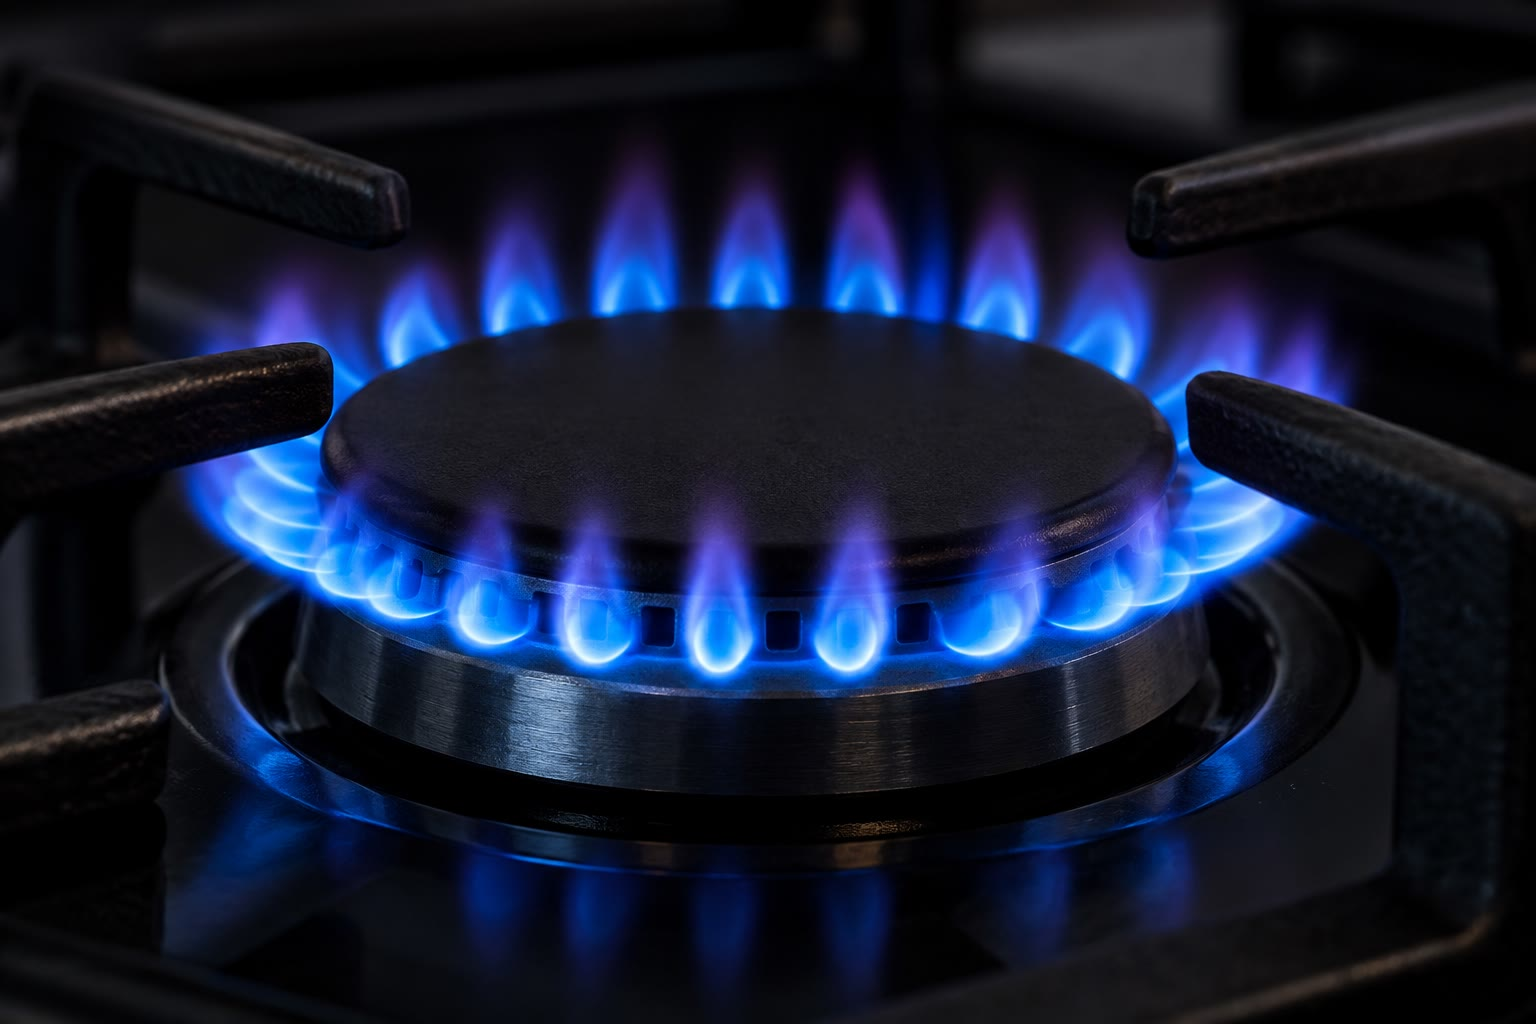
\includegraphics[width=0.5\linewidth]{images/book1/ai/g7-gas-flame.jpg}

{\small اللهب الأزرق لموقد الغاز: ميثان الغاز الطبيعي يحترق.}
\end{omfigure}

\section{النماذج الجزيئية}

\begin{remark}[النماذج وألوانها]\label{rem:g7:atoms-and-molecules:models}
يبني الكيميائيون \emph{نماذج جزيئية} من كرات تمثل \omterm{def:g7:atoms-and-molecules:atom}{الذرات} وعصيّ تمثل
الروابط بينها. والألوان اصطلاح متبع في العالم كله --- الكربون أسود،
والهيدروجين أبيض، والأكسجين أحمر، والنيتروجين أزرق --- وليست اللون
الحقيقي \omterm{def:g7:atoms-and-molecules:atom}{للذرات}: \omterm{def:g7:atoms-and-molecules:atom}{فالذرة} الواحدة لا لون لها أبدًا. ويبيّن النموذج أيضًا شكل
\omterm{def:g7:atoms-and-molecules:molecule}{الجزيء}، وهو ما لا تبيّنه الصيغة: \omterm{def:g7:atoms-and-molecules:molecule}{فجزيء} الماء منحنٍ، \omterm{def:g7:atoms-and-molecules:molecule}{وجزيء} ثنائي أكسيد
الكربون مستقيم.
\end{remark}

\begin{omfigure}
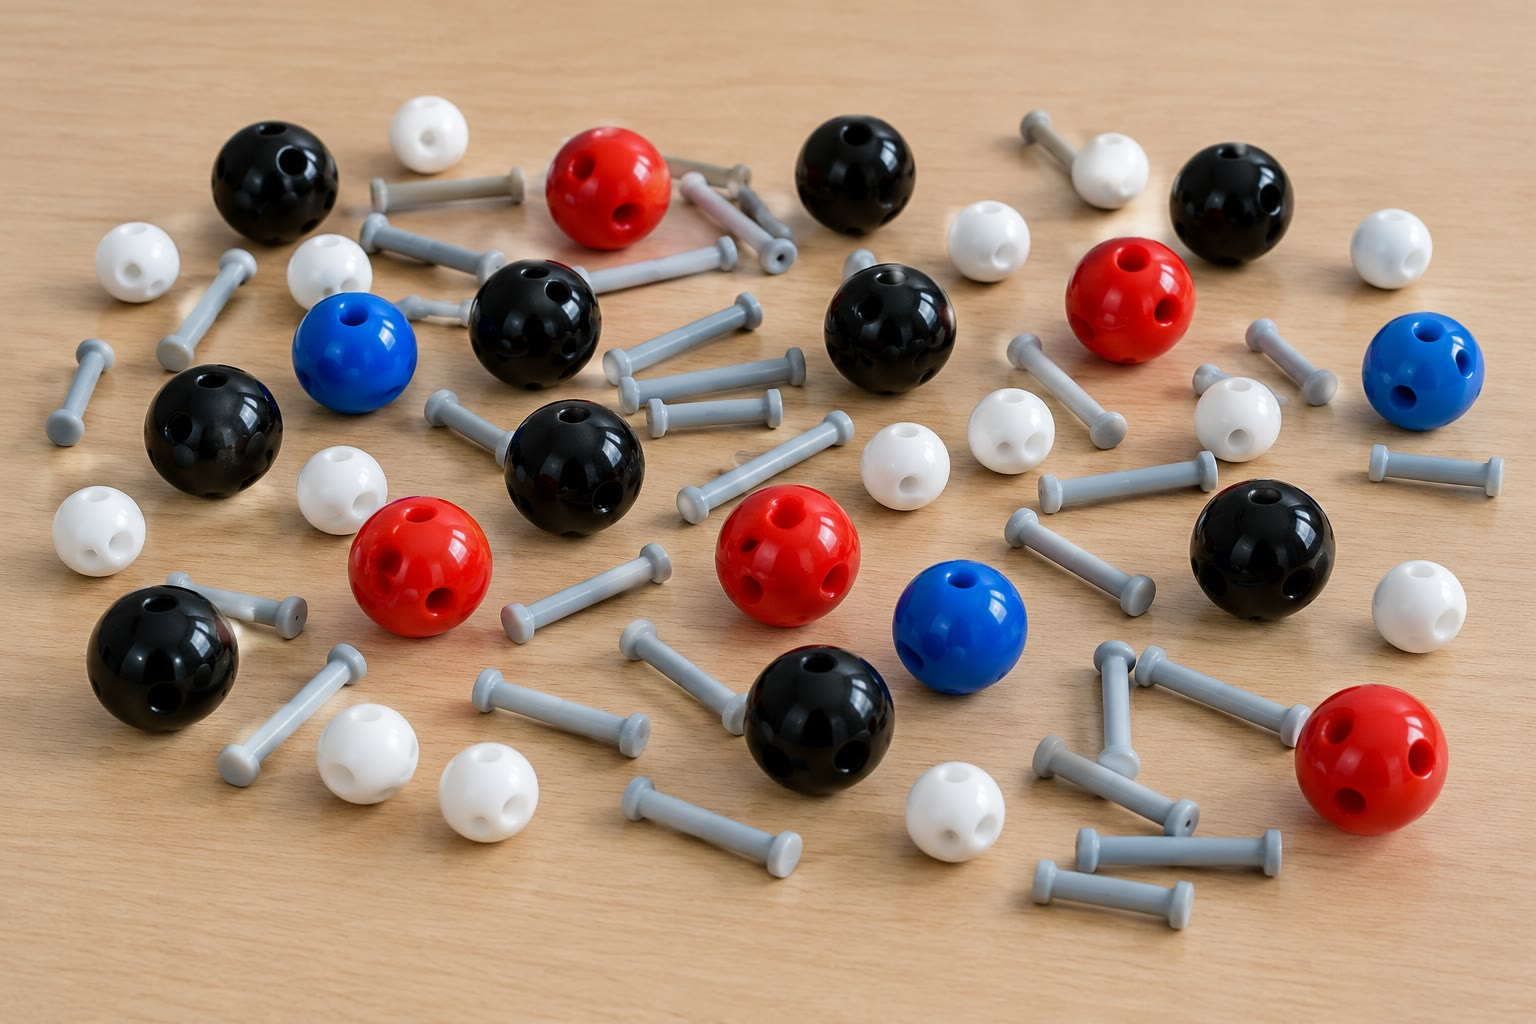
\includegraphics[width=0.5\linewidth]{images/book1/ai/g7-model-kit.jpg}

{\small طقم نماذج جزيئية: كرات تمثل \omterm{def:g7:atoms-and-molecules:atom}{الذرات}، فيها ثقوب للعصيّ التي
تمثل الروابط.}
\end{omfigure}

\begin{method}[من النموذج إلى الصيغة]\label{met:g7:atoms-and-molecules:model}
لكتابة صيغة \omterm{def:g7:atoms-and-molecules:molecule}{جزيء} انطلاقًا من نموذجه:
\begin{enumerate}
  \item سمِّ \omterm{def:g7:atoms-and-molecules:atom}{الذرات} من ألوانها؛
  \item عُدّ الكرات من كل لون؛
  \item اكتب الرموز مع الأعداد أدلةً سفلية، الكربون أولًا، ثم الهيدروجين،
        ثم \omterm{def:g7:atoms-and-molecules:atom}{الذرات} الأخرى بالترتيب الأبجدي اللاتيني
        لرموزها.
\end{enumerate}
كرة سوداء مرتبطة بأربع كرات بيضاء: كربون واحد، وأربعة هيدروجين:
\ce{CH4}.
\end{method}

\section{تمارين}

\begin{exercise}[$\star$]\label{exo:g7:atoms-and-molecules:1}
ما \omterm{def:g7:atoms-and-molecules:atom}{الذرة}؟ وما \omterm{def:g7:atoms-and-molecules:molecule}{الجزيء}؟
\end{exercise}

\begin{exercise}[$\star$]\label{exo:g7:atoms-and-molecules:2}
أعطِ رموز الهيدروجين، والكربون، والنيتروجين، والأكسجين، والصوديوم،
والحديد.
\end{exercise}

\begin{exercise}[$\star$]\label{exo:g7:atoms-and-molecules:3}
كم \omterm{def:g7:atoms-and-molecules:atom}{ذرة} من كل نوع في \omterm{def:g7:atoms-and-molecules:molecule}{جزيء} واحد من ثنائي أكسيد الكربون،
\ce{CO2}؟ وكم \omterm{def:g7:atoms-and-molecules:atom}{ذرة} في المجموع؟
\end{exercise}

\begin{exercise}[$\star$]\label{exo:g7:atoms-and-molecules:4}
سمِّ \omterm{def:g7:atoms-and-molecules:molecule}{الجزيئات} \ce{H2O} و\ce{O2} و\ce{CH4} و\ce{N2}.
\end{exercise}

\begin{exercise}[$\star$]\label{exo:g7:atoms-and-molecules:5}
\omterm{def:g7:atoms-and-molecules:molecule}{جزيء} ثنائي أكسيد النيتروجين، وهو غاز بني يوجد في \omterm{def:g4:air-a-mixture-of-gases:air}{الهواء} الملوث، مكوّن من
\omterm{def:g7:atoms-and-molecules:atom}{ذرة} نيتروجين واحدة وذرتي أكسجين. اكتب صيغته.
\end{exercise}

\begin{exercise}[$\star\star$]\label{exo:g7:atoms-and-molecules:6}
اشرح الفرق بين \ce{O2} و\ce{2O}، وبين \ce{CO}
و\ce{Co}.
\end{exercise}

\begin{exercise}[$\star\star$]\label{exo:g7:atoms-and-molecules:7}
كم \omterm{def:g7:atoms-and-molecules:atom}{ذرة} هيدروجين وكم \omterm{def:g7:atoms-and-molecules:atom}{ذرة} أكسجين في
\ce{3H2O}؟ وفي \ce{5O2}؟
\end{exercise}

\begin{exercise}[$\star\star$]\label{exo:g7:atoms-and-molecules:8}
نموذج مكوّن من كرة سوداء مرتبطة بكرتين حمراوين. سمِّ \omterm{def:g7:atoms-and-molecules:atom}{الذرات}، واكتب
الصيغة، وسمِّ \omterm{def:g7:atoms-and-molecules:molecule}{الجزيء}.
\end{exercise}

\begin{exercise}[$\star\star$]\label{exo:g7:atoms-and-molecules:9}
في جدول دالتون، الماء مكوّن من \omterm{def:g7:atoms-and-molecules:atom}{ذرة} هيدروجين واحدة \omterm{def:g7:atoms-and-molecules:atom}{وذرة} أكسجين واحدة.
اكتب الصيغة التي كان دالتون يتصورها، وقل كم \omterm{def:g7:atoms-and-molecules:atom}{ذرة} تنقص \omterm{def:g7:atoms-and-molecules:molecule}{جزيء} الماء
عنده.
\end{exercise}

\begin{exercise}[$\star\star$]\label{exo:g7:atoms-and-molecules:10}
هل الماء النقي \omterm{def:g6:pure-substances-and-mixtures:mixture}{خليط}؟ وهل \omterm{def:g4:air-a-mixture-of-gases:air}{الهواء} \omterm{def:g6:pure-substances-and-mixtures:mixture}{خليط}؟ أجب بوصف \omterm{def:g7:atoms-and-molecules:molecule}{الجزيئات} التي يحويها
كل منهما.
\end{exercise}

\begin{exercise}[$\star\star\star$]\label{exo:g7:atoms-and-molecules:11}
قطر \omterm{def:g7:atoms-and-molecules:atom}{ذرة} الهيدروجين نحو جزء من عشرة ملايين من المليمتر. كم \omterm{def:g7:atoms-and-molecules:atom}{ذرة} هيدروجين،
متراصفة جنبًا إلى جنب، تصنع خطًا طوله \qty{1}{cm}؟ وخطًا بطول ملعب كرة
القدم، \qty{100}{m}؟
\end{exercise}

\begin{exercise}[$\star\star\star$]\label{exo:g7:atoms-and-molecules:12}
الغلوكوز، السكر الذي يغذي خلايانا، صيغته
\ce{C6H12O6}. كم \omterm{def:g7:atoms-and-molecules:atom}{ذرة} يحوي \omterm{def:g7:atoms-and-molecules:molecule}{جزيء} غلوكوز واحد؟ وما النسبة المئوية \omterm{def:g7:atoms-and-molecules:atom}{لذرات}
الهيدروجين منها؟ وما النسبة المئوية \omterm{def:g7:atoms-and-molecules:atom}{لذرات} الكربون؟
\end{exercise}

\section{مسألة: ذرات نَفَس واحد}

\begin{problem}[{مسألة نهاية الأسبوع --- عدّ الذرات في نَفَس من الهواء،
قبل مروره في رئتينا وبعده}]
\label{pb:g7:atoms-and-molecules:1}
% ledger: air:N2, air:O2, air:Ar (78.08 / 20.95 / 0.93 rounded to 78 / 21 / 1),
% breath:O2, breath:CO2, breath:N2 (expired air: 16 / 4 / 78, water vapour removed)
يمر النيتروجين في الرئتين دون أن يتغير، فهو مقياس مرجعي جيد. ففي \omterm{def:g4:air-a-mixture-of-gases:air}{الهواء}
الجاف، لكل 78 \omterm{def:g7:atoms-and-molecules:molecule}{جزيء} نيتروجين نحو 21 \omterm{def:g7:atoms-and-molecules:molecule}{جزيء} أكسجين \omterm{def:g7:atoms-and-molecules:atom}{وذرة} أرغون واحدة: أي
100 جسيم (\omterm{def:g7:atoms-and-molecules:molecule}{جزيئات} أو \omterm{def:g7:atoms-and-molecules:atom}{ذرات} منفردة) في المجموع. وفي \omterm{def:g4:air-a-mixture-of-gases:air}{هواء} الزفير، بعد
نزع بخار الماء منه، تصحب \omterm{def:g7:atoms-and-molecules:molecule}{جزيئات} النيتروجين نفسها، وعددها 78، نحو 16 \omterm{def:g7:atoms-and-molecules:molecule}{جزيء}
أكسجين، و4 \omterm{def:g7:atoms-and-molecules:molecule}{جزيئات} ثنائي أكسيد الكربون، \omterm{def:g7:atoms-and-molecules:atom}{وذرة} أرغون واحدة.

\medskip
\noindent\textbf{الجزء الأول --- \omterm{def:g4:air-a-mixture-of-gases:air}{الهواء} الذي نستنشقه.}
\begin{enumerate}
  \item اكتب صيغ \omterm{def:g7:atoms-and-molecules:molecule}{جزيئات} النيتروجين والأكسجين وثنائي أكسيد الكربون، وأعطِ
        عدد \omterm{def:g7:atoms-and-molecules:atom}{الذرات} في كل منها.
  \item يُعدّ الأرغون \omterm{def:g7:atoms-and-molecules:atom}{بالذرات} لا \omterm{def:g7:atoms-and-molecules:molecule}{بالجزيئات}. ماذا يخبرنا هذا عن
        الأرغون؟
  \item في هذه الجسيمات المئة من \omterm{def:g4:air-a-mixture-of-gases:air}{هواء} الشهيق، كم \omterm{def:g7:atoms-and-molecules:atom}{ذرة} نيتروجين
        توجد؟ وكم \omterm{def:g7:atoms-and-molecules:atom}{ذرة} أكسجين؟
  \item كم \omterm{def:g7:atoms-and-molecules:atom}{ذرة} توجد في المجموع في هذه الجسيمات المئة؟
  \item ما النسبة المئوية \omterm{def:g7:atoms-and-molecules:atom}{لذرات} النيتروجين من هذه \omterm{def:g7:atoms-and-molecules:atom}{الذرات}؟ قرّب إلى أقرب
        عدد صحيح.
\end{enumerate}

\medskip
\noindent\textbf{الجزء الثاني --- \omterm{def:g4:air-a-mixture-of-gases:air}{الهواء} الذي نزفره.}
\begin{enumerate}[resume]
  \item في \omterm{def:g4:air-a-mixture-of-gases:air}{هواء} الزفير المرافق \omterm{def:g7:atoms-and-molecules:molecule}{لجزيئات} النيتروجين نفسها (78 جزيئًا)، كم \omterm{def:g7:atoms-and-molecules:atom}{ذرة}
        أكسجين داخل \omterm{def:g7:atoms-and-molecules:molecule}{جزيئات} الأكسجين؟ وكم داخل \omterm{def:g7:atoms-and-molecules:molecule}{جزيئات} ثنائي أكسيد
        الكربون؟ وكم في المجموع؟
  \item قارن بالسؤال 3. كم \omterm{def:g7:atoms-and-molecules:atom}{ذرة} أكسجين تنقص؟ وإلى أي \omterm{def:g7:atoms-and-molecules:molecule}{جزيء} ذهبت، وهو
        \omterm{def:g7:atoms-and-molecules:molecule}{جزيء} يُصنع في الجسم من هيدروجين الغذاء ويُنزع هنا مع بخار
        الماء؟
  \item كم \omterm{def:g7:atoms-and-molecules:atom}{ذرة} كربون في \omterm{def:g4:air-a-mixture-of-gases:air}{هواء} الشهيق؟ وكم في \omterm{def:g4:air-a-mixture-of-gases:air}{هواء}
        الزفير؟
  \item \omterm{def:g4:air-a-mixture-of-gases:air}{الهواء} لا يُدخل أي \omterm{def:g7:atoms-and-molecules:atom}{ذرة} كربون إلى الرئتين. فمن أين يمكن أن تأتي
        \omterm{def:g7:atoms-and-molecules:atom}{ذرات} الكربون في النَّفَس؟ (فكّر فيما يستعمله الجسم
        ليعيش.)
  \item كم \omterm{def:g7:atoms-and-molecules:molecule}{جزيء} أكسجين اختفى، وكم \omterm{def:g7:atoms-and-molecules:molecule}{جزيء} ثنائي أكسيد كربون
        ظهر؟
\end{enumerate}

\medskip
\noindent\textbf{الجزء الثالث --- الحساب.}
\begin{enumerate}[resume]
  \item صف نموذج الكرات والعصيّ لكل نوع من أنواع الجسيمات الأربعة في
        \omterm{def:g4:air-a-mixture-of-gases:air}{هواء} الزفير، مع ألوان الكرات (يمثَّل الأرغون بكرة واحدة زرقاء
        فاتحة).
  \item كم \omterm{def:g7:atoms-and-molecules:atom}{ذرة} في المجموع في \omterm{def:g4:air-a-mixture-of-gases:air}{هواء} الزفير المجفف؟ وبكم \omterm{def:g7:atoms-and-molecules:atom}{ذرة} يزيد على \omterm{def:g4:air-a-mixture-of-gases:air}{هواء}
        الشهيق؟ فسّر الفرق \omterm{def:g7:atoms-and-molecules:atom}{بذرات} الكربون المكتسبة \omterm{def:g7:atoms-and-molecules:atom}{وذرات} الأكسجين
        الناقصة.
\end{enumerate}
\end{problem}
